\RequirePackage[l2tabu, orthodox, abort]{nag}
\documentclass[a4paper, 11pt]{article}

\usepackage[utf8x]{inputenc}
\usepackage[T1]{fontenc}
\usepackage{ucs}
\usepackage[english]{babel}
\usepackage{mathtools, amsmath, amsfonts, amssymb}
\usepackage{fancyhdr}
\usepackage[parfill]{parskip}
\usepackage{graphicx}
\usepackage[sc]{mathpazo}
\usepackage[scaled]{beramono}
\usepackage[scaled]{helvet}
\usepackage{float}
\usepackage{array}
\usepackage{booktabs}
\usepackage[font={small,it}]{caption}
\usepackage{fixltx2e}
\usepackage[colorinlistoftodos]{todonotes}
\usepackage{bm}
\usepackage{xfrac}
% \usepackage{fullpage}

\linespread{1.05}
\pagestyle{fancyplain}
\fancyhead{}
\fancyfoot[L]{}
\fancyfoot[C]{}
\fancyfoot[R]{\thepage}
\renewcommand{\headrulewidth}{0pt}
\renewcommand{\footrulewidth}{0pt}
\setlength{\headheight}{13.6pt}

\widowpenalty=1000
\clubpenalty=1000

\newcommand{\horrule}[1]{\rule{\linewidth}{#1}}
\newcommand{\vect}[1]{\mathbf{#1}}
\newcommand{\mat}[1]{\textbf{#1}}

% Todonotes commands.
\newcommand{\addref}{\todo[color=red!40]{Add reference.}}
\newcommand{\rewrite}[1]{\todo[color=green!40]{#1}} 
\newcommand{\missing}[1]{\todo[inline,color=green!40]{Need to write: #1}}

\title{ 
\normalfont\normalsize 
\textsc{University of Copenhagen} \\ [25pt]
\horrule{0.5pt} \\[0.4cm]
\huge StatML\@: Exam 2014\\
\horrule{2pt} \\[0.5cm]
}

\author{Jens Fredskov (chw752)}

\begin{document}
\maketitle
\pagebreak

\section{Predicting the Specific Star Formation Rate} % (fold)
\label{sec:predicting_the_specific_star_formation_rate}

\subsection*{Question 1}

\[
    \mathbf{w}_{\mathit{ML}} = \begin{pmatrix}
      -8.1494 \\
       -0.794 \\
       -1.223 \\
     -0.32858 \\
     -0.78633 \\
    \end{pmatrix}
\]

\begin{align*}
    \mathrm{MSE}_{\mathit{train}} &= 0.27475 \\
    \mathrm{MSE}_{\mathit{test}} &= 0.27518
\end{align*}

Notes: we could also do regularization, and/or radial/polynomial basis functions.
Source code: question1.m linearRegression.m meanSquaredError.m

\subsection*{Question 2}
Source code: question2.m, polyRegression.m, polyPredict.m, meanSquaredError.m, betterPlots.m

\begin{figure}[H]
    \centering
    \includegraphics[width=0.8\textwidth]{figures/question2}
    \caption{Here be dragons.}\label{fig:question2}
\end{figure}

degree of polynimium = 3

\begin{align*}
    \mathrm{MSE}_{\mathit{train}} &= 0.25635 \\
    \mathrm{MSE}_{\mathit{test}} &= 0.25835
\end{align*}

% section predicting_the_specific_star_formation_rate (end)

\section{Stars vs. Galaxies} % (fold)
\label{sec:stars_vs_galaxies}

\subsection*{Question 3}

Notes: $\sigma = \sqrt{1 / (2 \gamma)} \Leftrightarrow \gamma = 1 / (2 \sigma^2)$

\[
    \sigma_{\mathit{jaakkola}} = 1.8119 \quad \gamma_{\mathit{jaakkola}} = 0.1523
\]

\[
    C_{\mathit{best}} = 1000 \quad \sigma_{\mathit{best}} = 0.001523
\]

\begin{align*}
    \mathrm{Accuracy}_{\mathit{train}} &= 0.997333 \\
    \mathrm{Accuracy}_{\mathit{test}} &= 0.996333
\end{align*}

Source code: question3.m jaakkola.m crossValidation.m svmClassify.m

Notes: used SVMLIB

\subsection*{Question 4}

\begin{figure}[H]
    \centering
    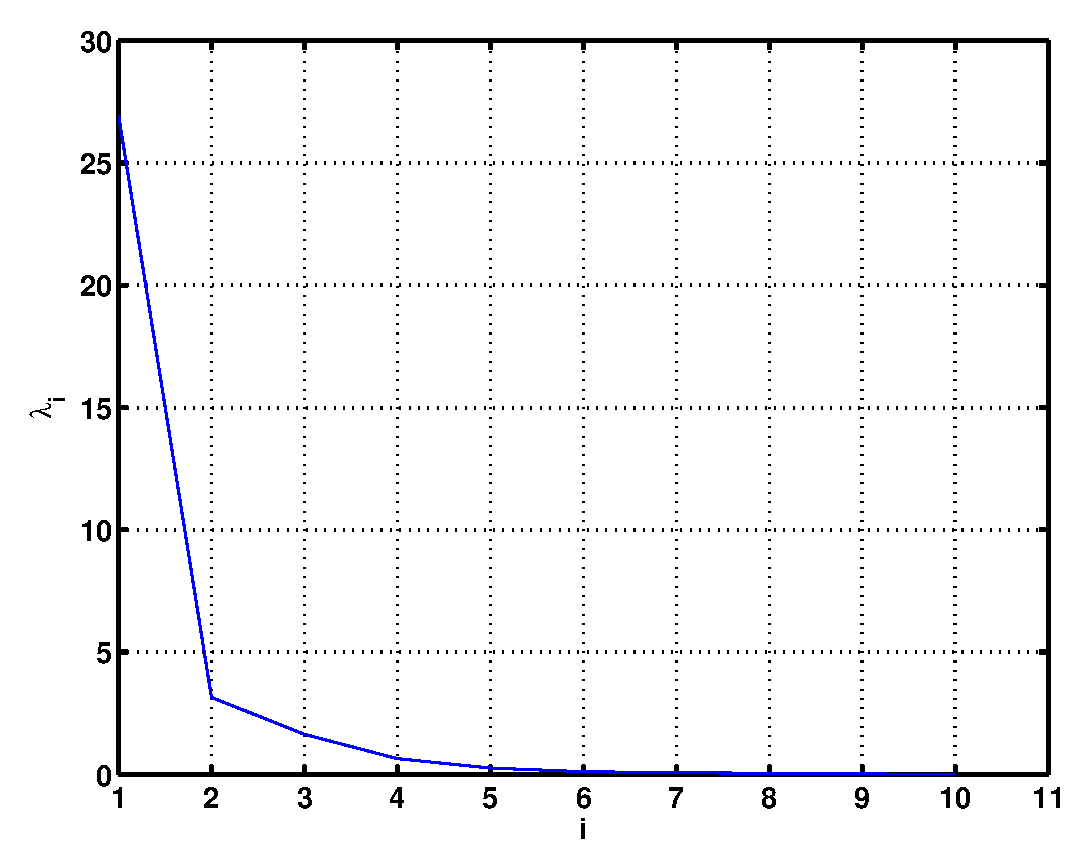
\includegraphics[width=0.8\textwidth]{figures/question4_1}
    \caption{Here be dragons.}\label{fig:question4_1}
\end{figure}

\begin{figure}[H]
    \centering
    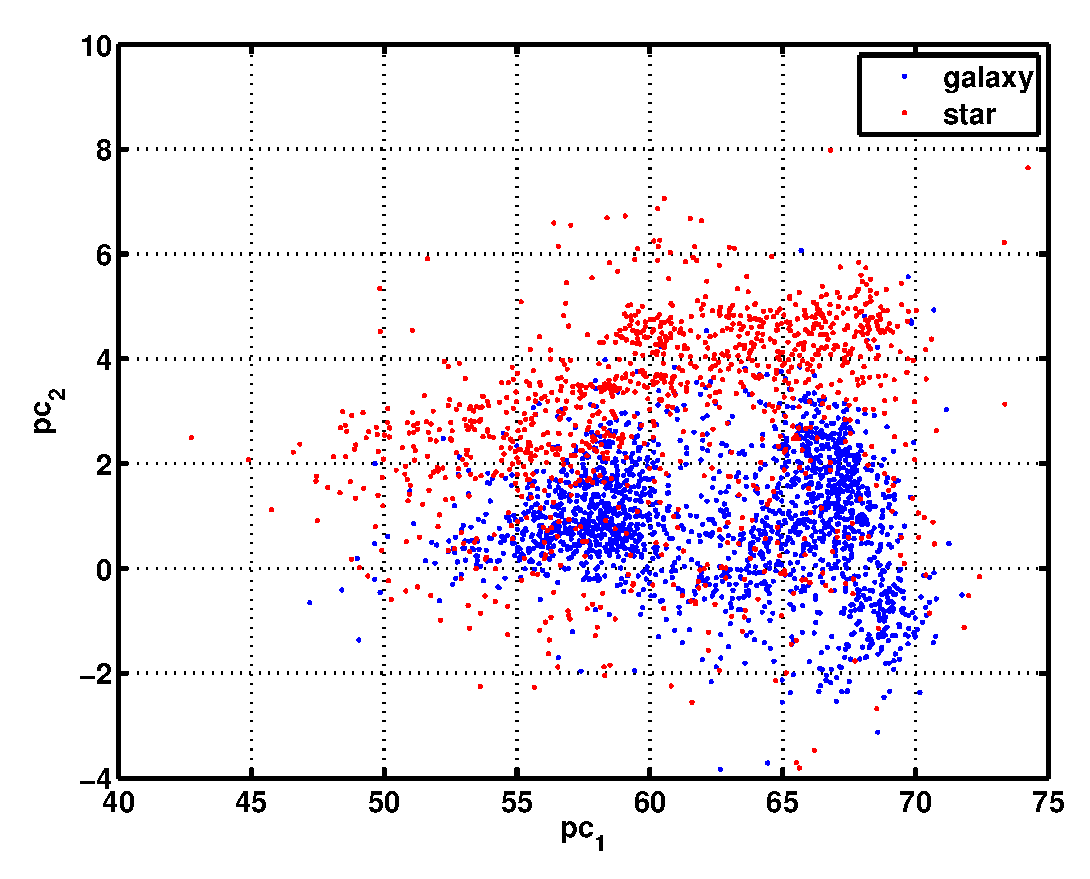
\includegraphics[width=0.8\textwidth]{figures/question4_2}
    \caption{Here be dragons.}\label{fig:question4_2}
\end{figure}

Source code: question4.m pca.m, betterPlots.m

\subsection*{Question 5}

\[
    c_1 = \begin{pmatrix}
       19.324 \\
       17.971 \\
       17.291 \\
       16.965 \\
       16.774 \\
       20.297 \\
       18.876 \\
       18.201 \\
       17.880 \\
       17.647 \\
    \end{pmatrix} \quad
    c2 = \begin{pmatrix}
       22.349 \\
       21.413 \\
       20.290 \\
       19.599 \\
       19.222 \\
       23.451 \\
       22.096 \\
       20.946 \\
       20.272 \\
       19.855 \\
    \end{pmatrix}
\]

\begin{figure}[H]
    \centering
    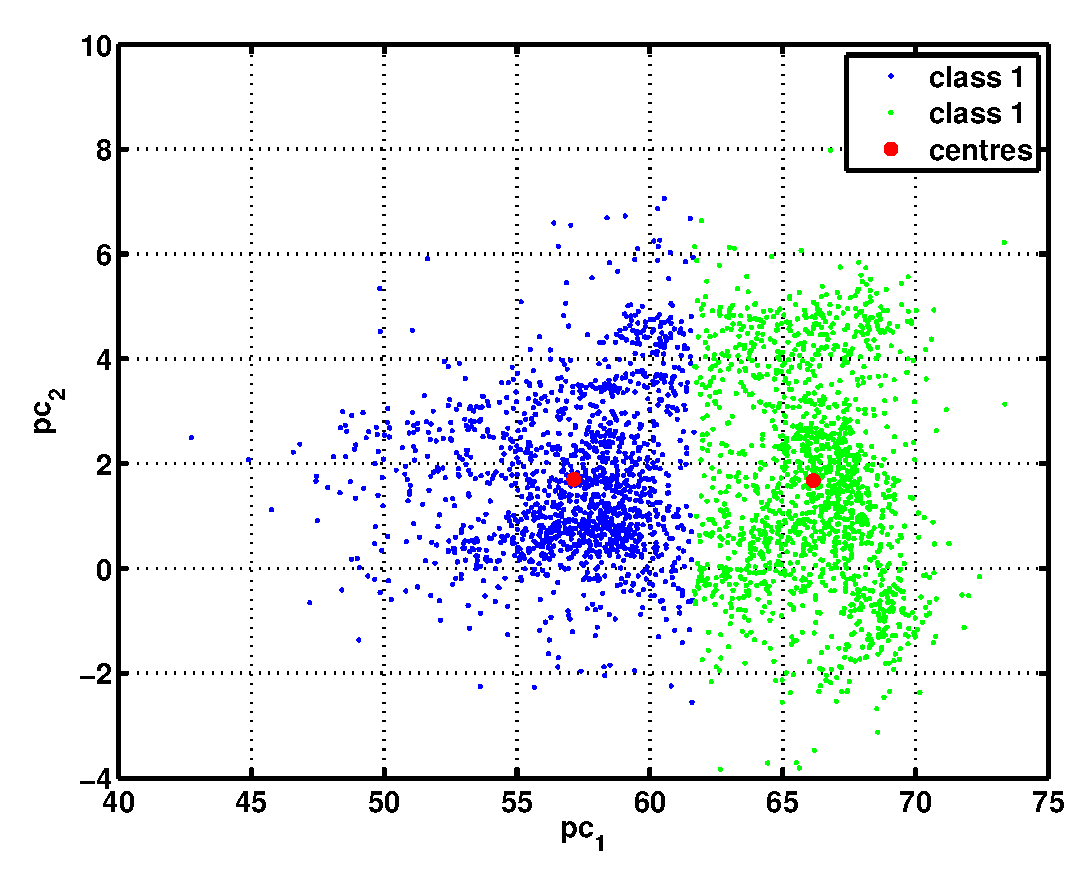
\includegraphics[width=0.8\textwidth]{figures/question5_1}
    \caption{Here be dragons.}\label{fig:question5_1}
\end{figure}

Source code: question5.m, betterPlots.m

Notes: used built-in kmeans from MATLAB

\subsection*{Question 6}

% section stars_vs_galaxies (end)

\section{Variable Stars} % (fold)
\label{sec:variable_stars}

\subsection*{Question 7}

Linear classification
\begin{align*}
    E_{\mathit{train}} &= 0.18418 \\
    E_{\mathit{test}} &= 0.28664
\end{align*}

Nonlinear classification
\[
    k_{\mathit{best}} = 6
\]
\begin{align*}
    E_{\mathit{train}} &= 0.44877 \\
    E_{\mathit{test}} &= 0.55512
\end{align*}


Notes: used LDA and KNN\@. KNN used 5-fold cross-val to choose K
Source code: question7.m trainLDA.m kNN.m crossValidation.m

\subsection*{Question 8}

% section variable_stars (end)

\end{document}